%\chapter*{Неделя 13}
\protect\thispagestyle{fancy}
\section{}
Для нерекурсивного фильтра первого порядка, заданного разностным уравнением
\begin{equation*}
	y[k] = x[k] + ax[k-1]
\end{equation*}

найти значения $a$, при которых

\begin{enumerate}[label=(\alph*)]
	\item для всех частот одинаковая фазовая задержка $\tau_{ph}(\theta) = \text{const}$,
	\item для всех частот одинаковая групповая задержка $\tau_{gr}(\theta) = \text{const}$.
\end{enumerate}

Изобразить ФЧХ для этих случаев на отрезке $\theta \in [-\pi; \pi]$.

\begin{gather*}
	\Capit{H}(z) = 1 + az^{-1}\big|_{z = e^{j \theta}} = 1 + ae^{-j \theta} =
	(1 + a\cos\theta) -ja\sin\theta,\quad \Rightarrow
	\varphi(\theta) = \arg\{\Capit{H}(\theta)\} = -\text{arctg}\left(\frac{a\sin\theta}{1+a\cos\theta}\right).
\end{gather*}

\begin{align*}
	\tau_{ph}(\theta) = -\dfrac{\varphi(\theta)}{\theta}\Delta t = \dfrac{\Delta t}{\theta}\text{arctg}\left(\frac{a\sin\theta}{1+a\cos\theta}\right),\quad
	\tau_{gr}(\theta) = -\dfrac{d\varphi(\theta)}{d\theta}\Delta t = \Delta t \dfrac{d}{d\theta} \left\{ \text{arctg}\left(\frac{a\sin\theta}{1+a\cos\theta}\right) \right\}.
\end{align*}

\begin{gather*}
	\tau_{ph}(\theta) = \text{const} \Leftrightarrow a \in \{0, 1\},\\
	\tau_{gr}(\theta) = \text{const} \Leftrightarrow a \in \{-1, 0, 1\}.
\end{gather*}

\begin{figure}[!h]
	\centering
	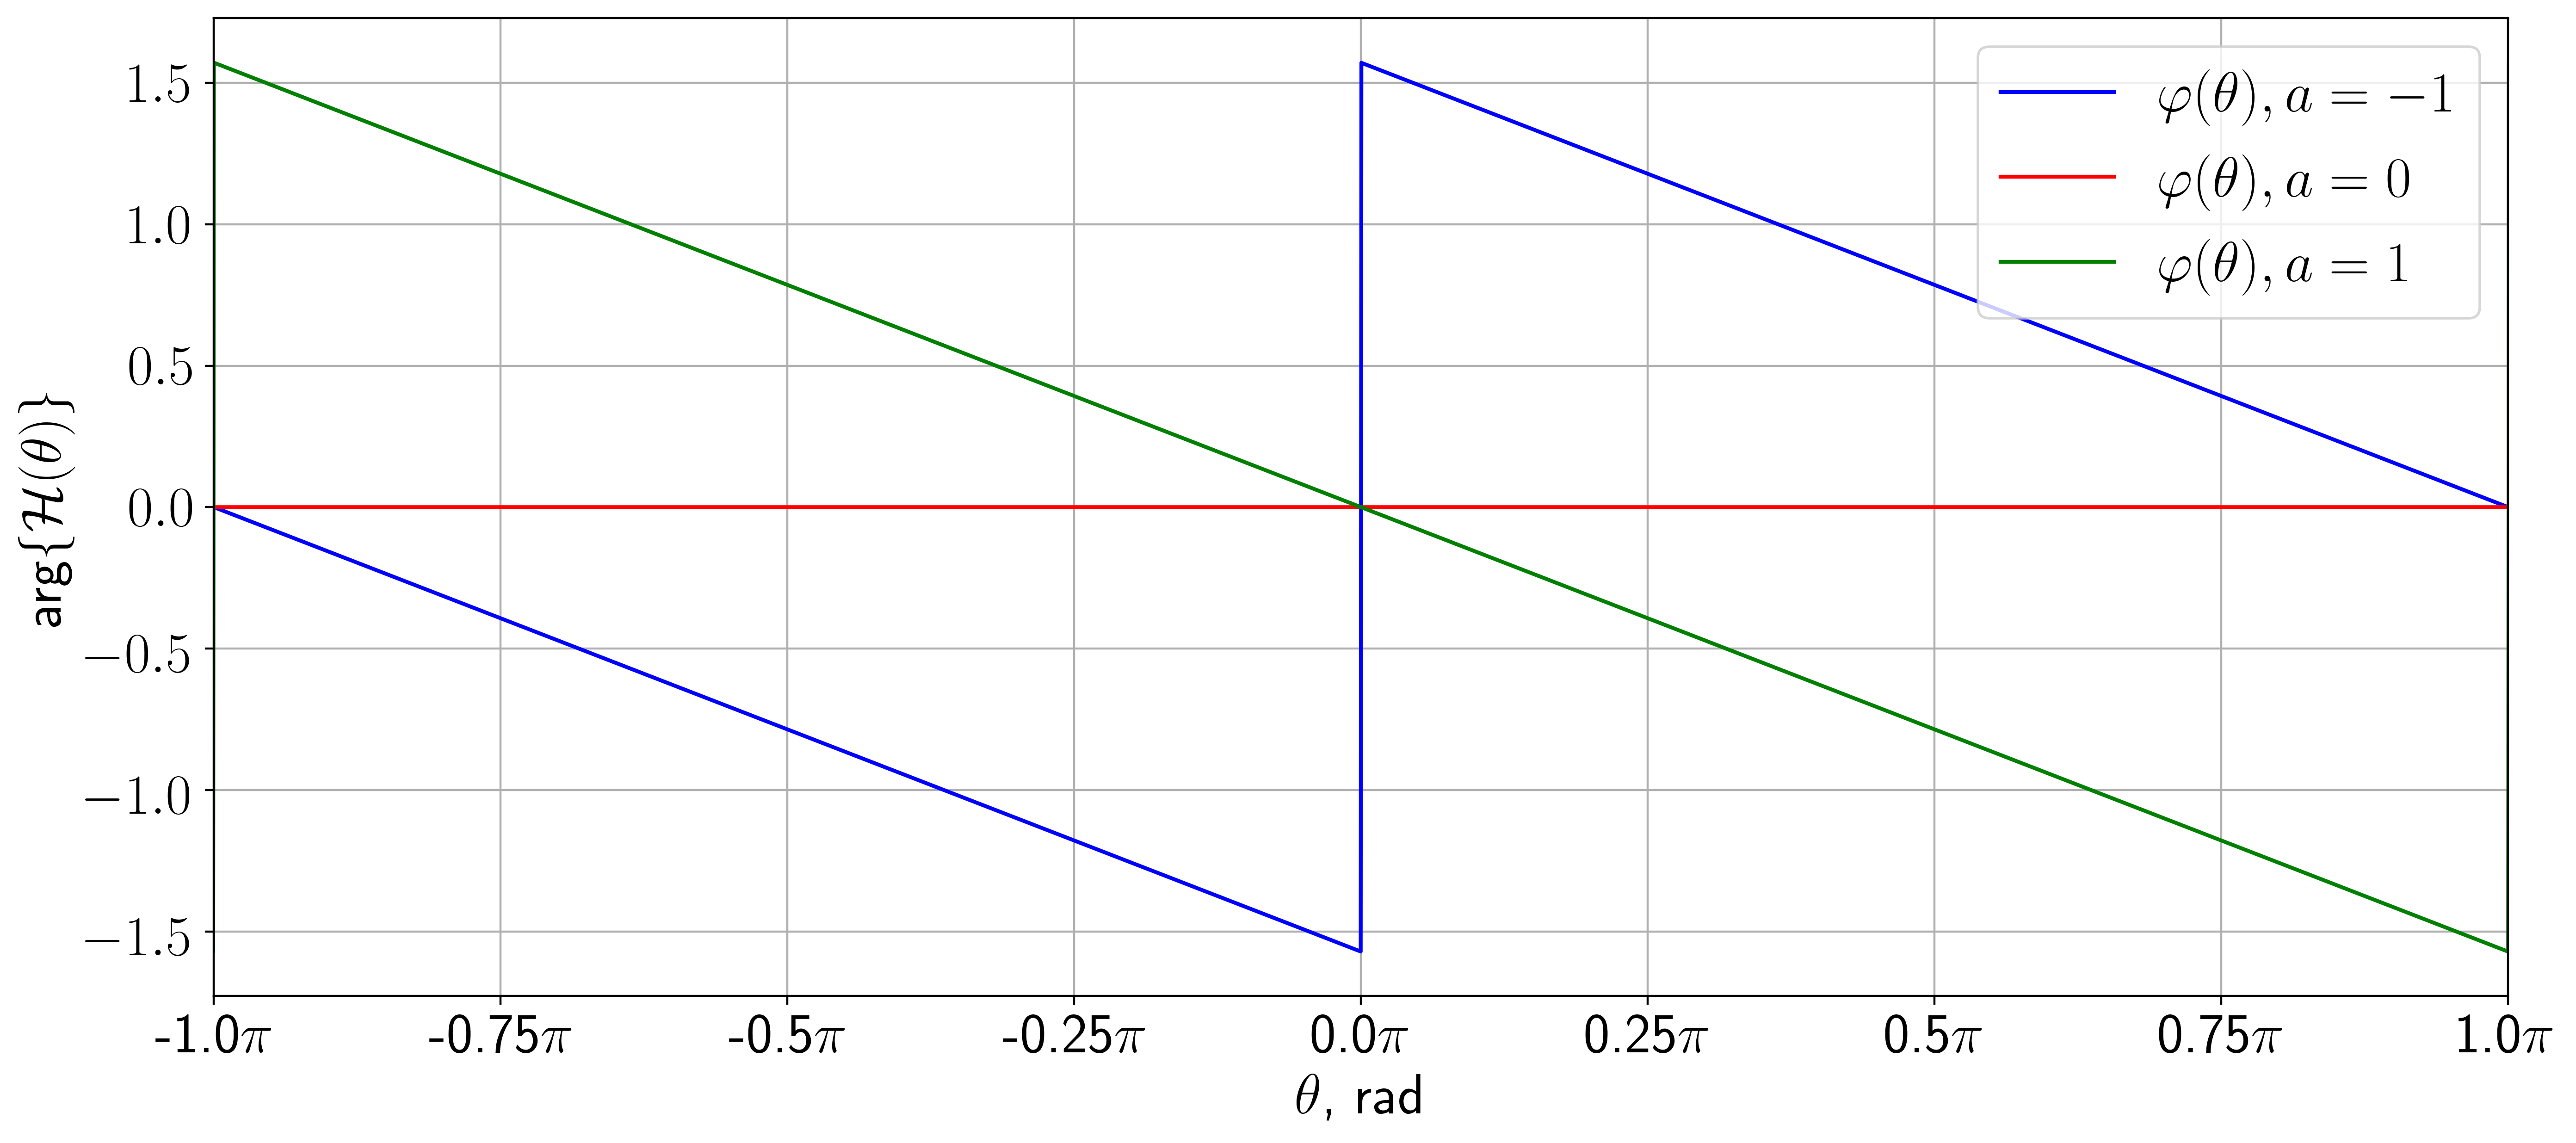
\includegraphics[width=0.8\columnwidth]{pics/fall/13/13-1.png}
	\label{fig:13-1}
\end{figure}


\newpage
\section{}

Определить АЧХ и ФЧХ гребенчатого фильтра $y[k] = x[k] - x[k-N]$.
Является ли ФЧХ линейной?

\begin{equation*}
	\Capit{H}(z) = 1 - z^{-N}\big|_{z = e^{j \theta}} = 1 - \exp\big(-jN \theta \big) =
	2 j\exp\Big(-j \frac{N \theta}{2}\Big) \sin\Big(\frac{N \theta}{2}\Big) =
	2 \exp\Big(j \Big(\frac{\pi}{2} - \frac{N \theta}{2}\Big)\Big) \sin\Big(\frac{N \theta}{2}\Big).
\end{equation*}

\begin{gather*}
	|\Capit{H}(\theta)| = 2\Big|\sin\Big(\frac{N \theta}{2}\Big)\Big|,\\
	\varphi(\theta) = \frac{\pi}{2} - \frac{N \theta}{2},\;\text{где } 0 \leq \theta \leq \frac{2\pi}{N} \text{ с периодом } T_{\theta} = \dfrac{2\pi}{N}.\quad \text{(С учётом смены знака синусом.)}
\end{gather*}

ФЧХ данного фильтра является линейной (кусочно-линейной).

\begin{figure}[!h]
	\centering
	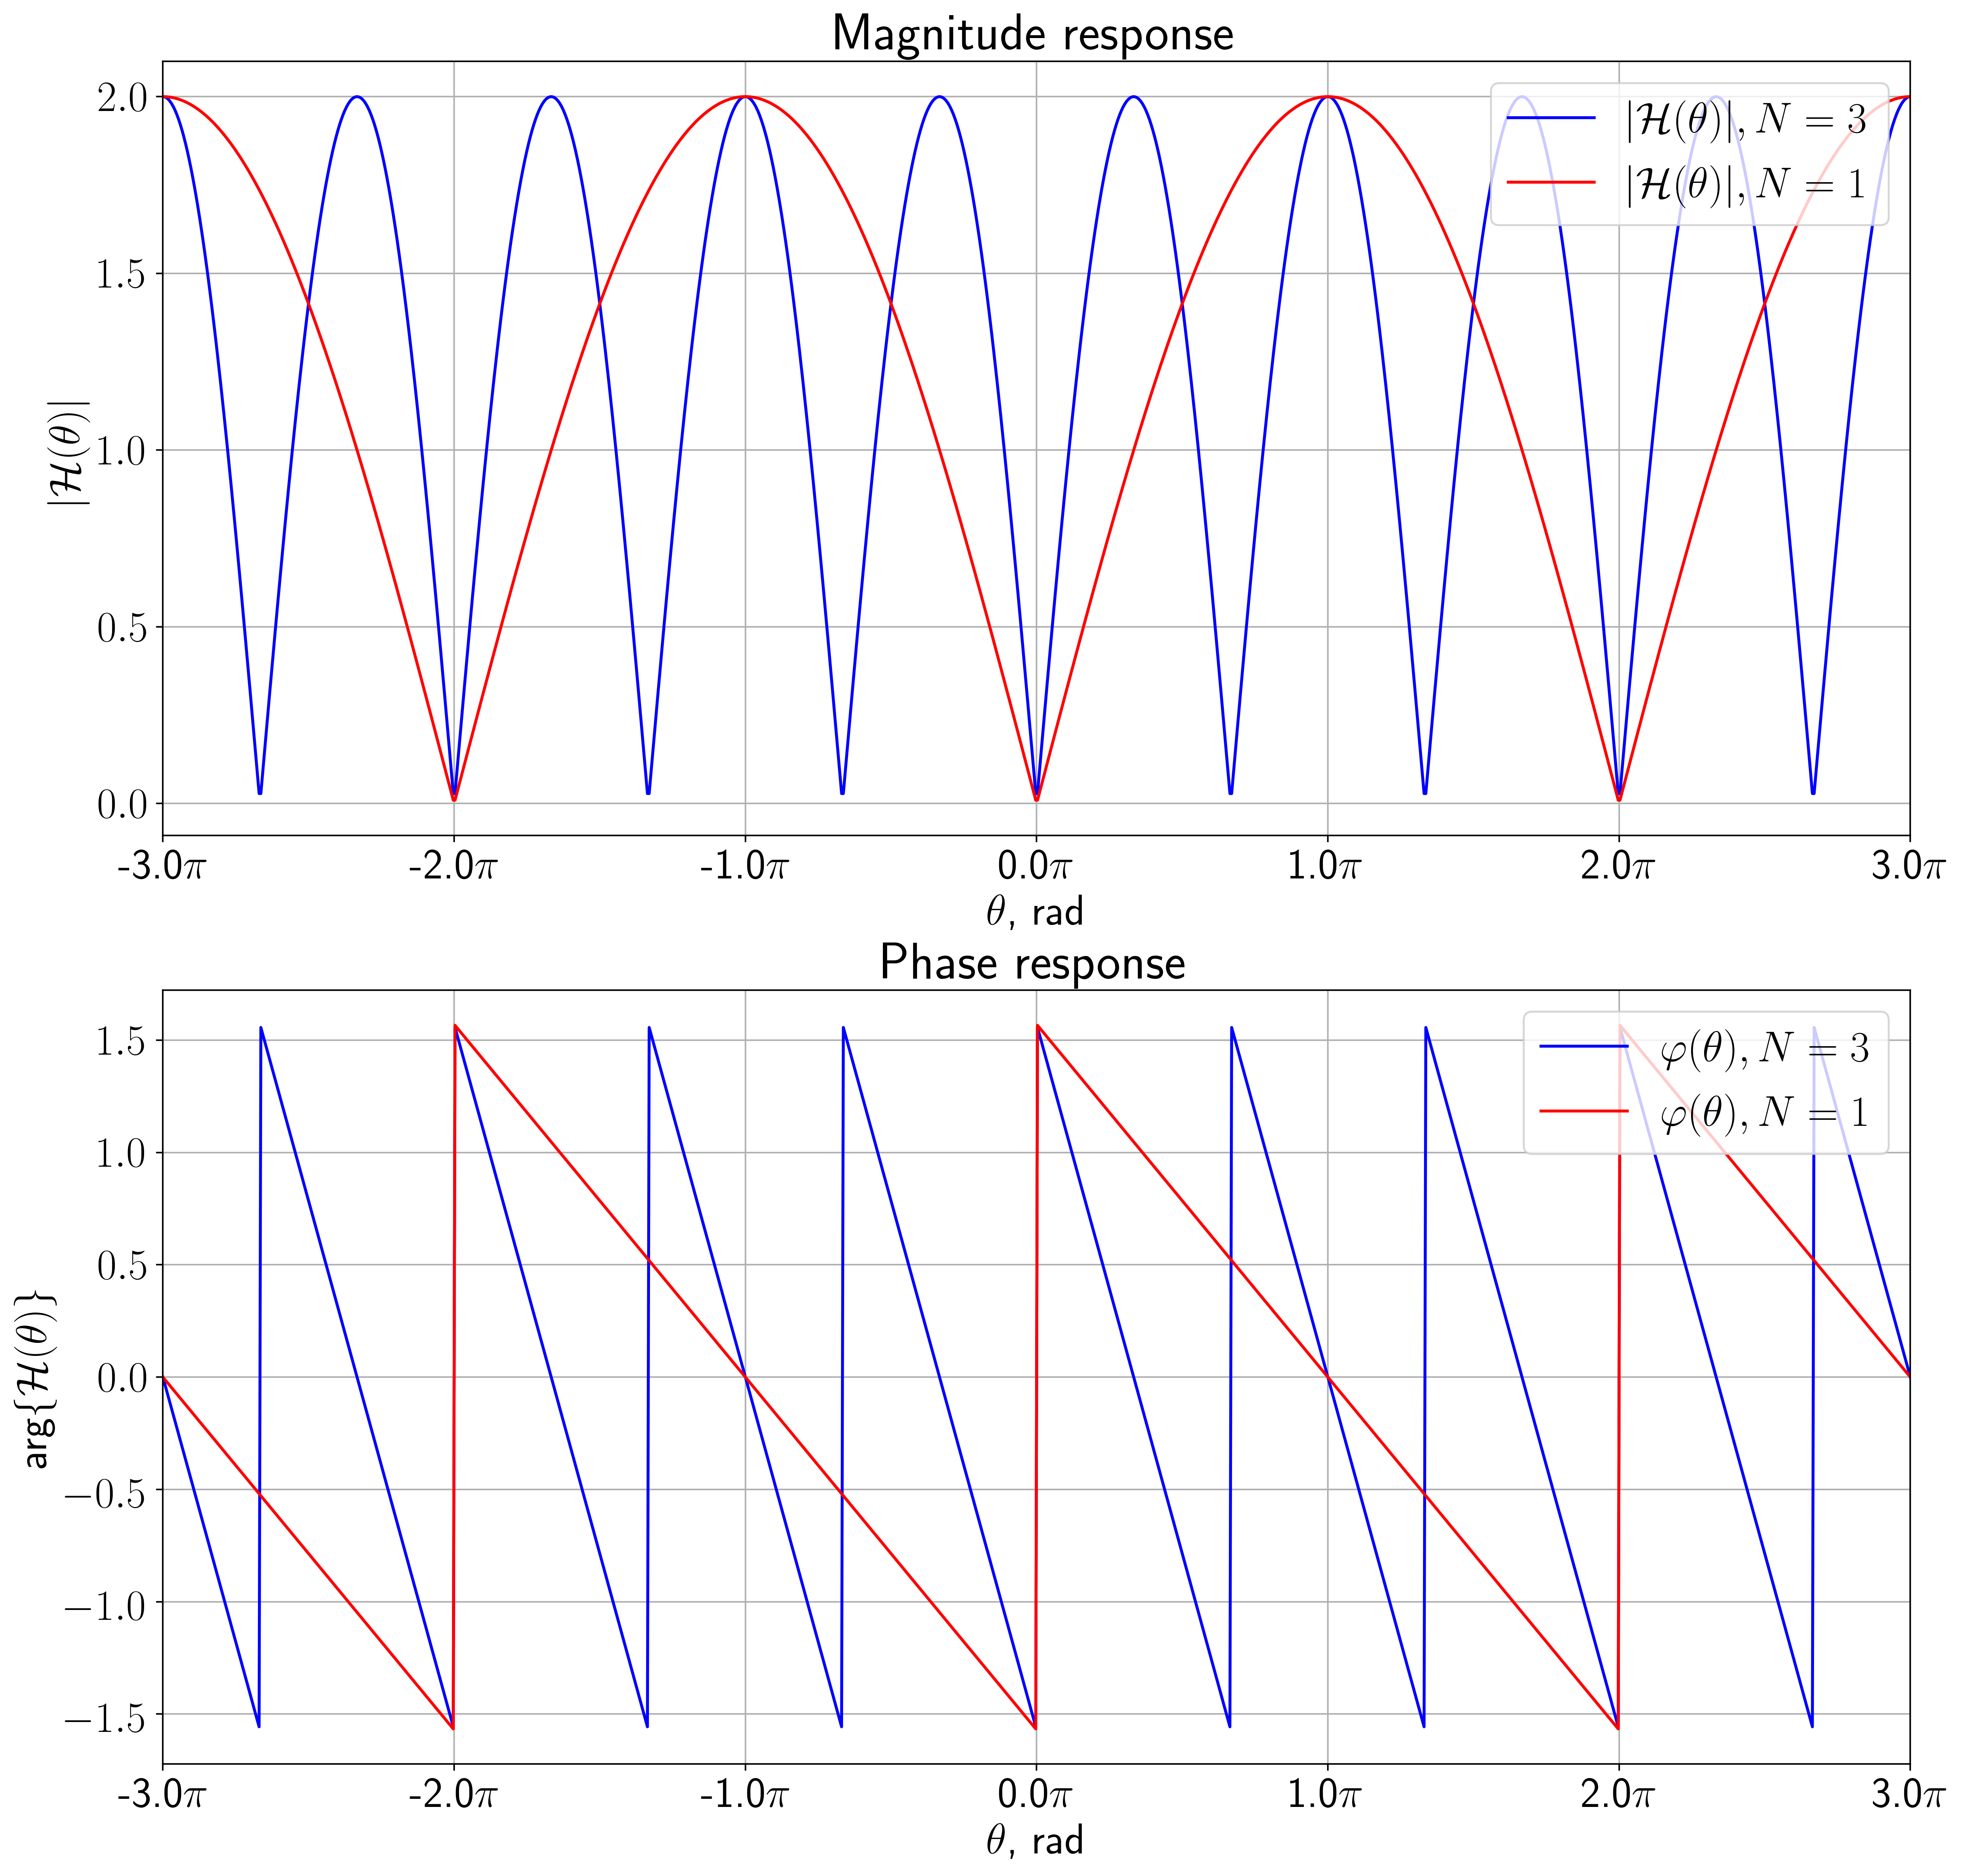
\includegraphics[width=0.8\columnwidth]{pics/fall/13/13-2.png}
	\label{fig:13-2}
\end{figure}


\newpage
\section{}

Определить ФЧХ CIC-фильтра с передаточной функцией
\begin{equation*}
	\Capit{H}_2(z) = \left(\dfrac{1 - z^{-N}}{1 - z^{-1}}\right)^2.
\end{equation*}

Будет ли ФЧХ такого фильтра линейной на $\theta \in [-\pi; \pi]$?
Как это соотносится с видом импульсной характеристики такого фильтра?

\begin{equation*}
	\Capit{H}_2(z) = \left(\dfrac{1 - z^{-N}}{1 - z^{-1}}\right)^2\Big|_{z = e^{j \theta}} =
	\left(\dfrac{1 - e^{-jN\theta}}{1 - e^{-j\theta}}\right)^2 =
	\dfrac{e^{-jN\theta}}{e^{-j\theta}} \dfrac{\sin^2\left(\frac{N \theta}{2}\right)}{\sin^2\left(\frac{\theta}{2}\right)} =
	e^{-j(N-1)\theta} \cdot \dfrac{\sin^2\left(\frac{N \theta}{2}\right)}{\sin^2\left(\frac{\theta}{2}\right)}.
\end{equation*}

\begin{equation*}
	\varphi(\theta) = -j(N-1)\theta + \frac{2\pi}{(N-1)}m,\; m \in \mathbb{Z}.
\end{equation*}

ФЧХ данного фильтра является линейной (кусочно-линейной). Это означает, что импульсная характеристика должна иметь симметричный или антисимметричный вид.
Действительно, импульсная характеристика данного фильтра содержит $2N-1$ ненулевых отсчётов и является дискретной свёрткой двух последовательностей единичных импульсов длины $N$. Такая свёртка имеет симметричный треугольный вид.

\begin{figure}[!h]
	\centering
	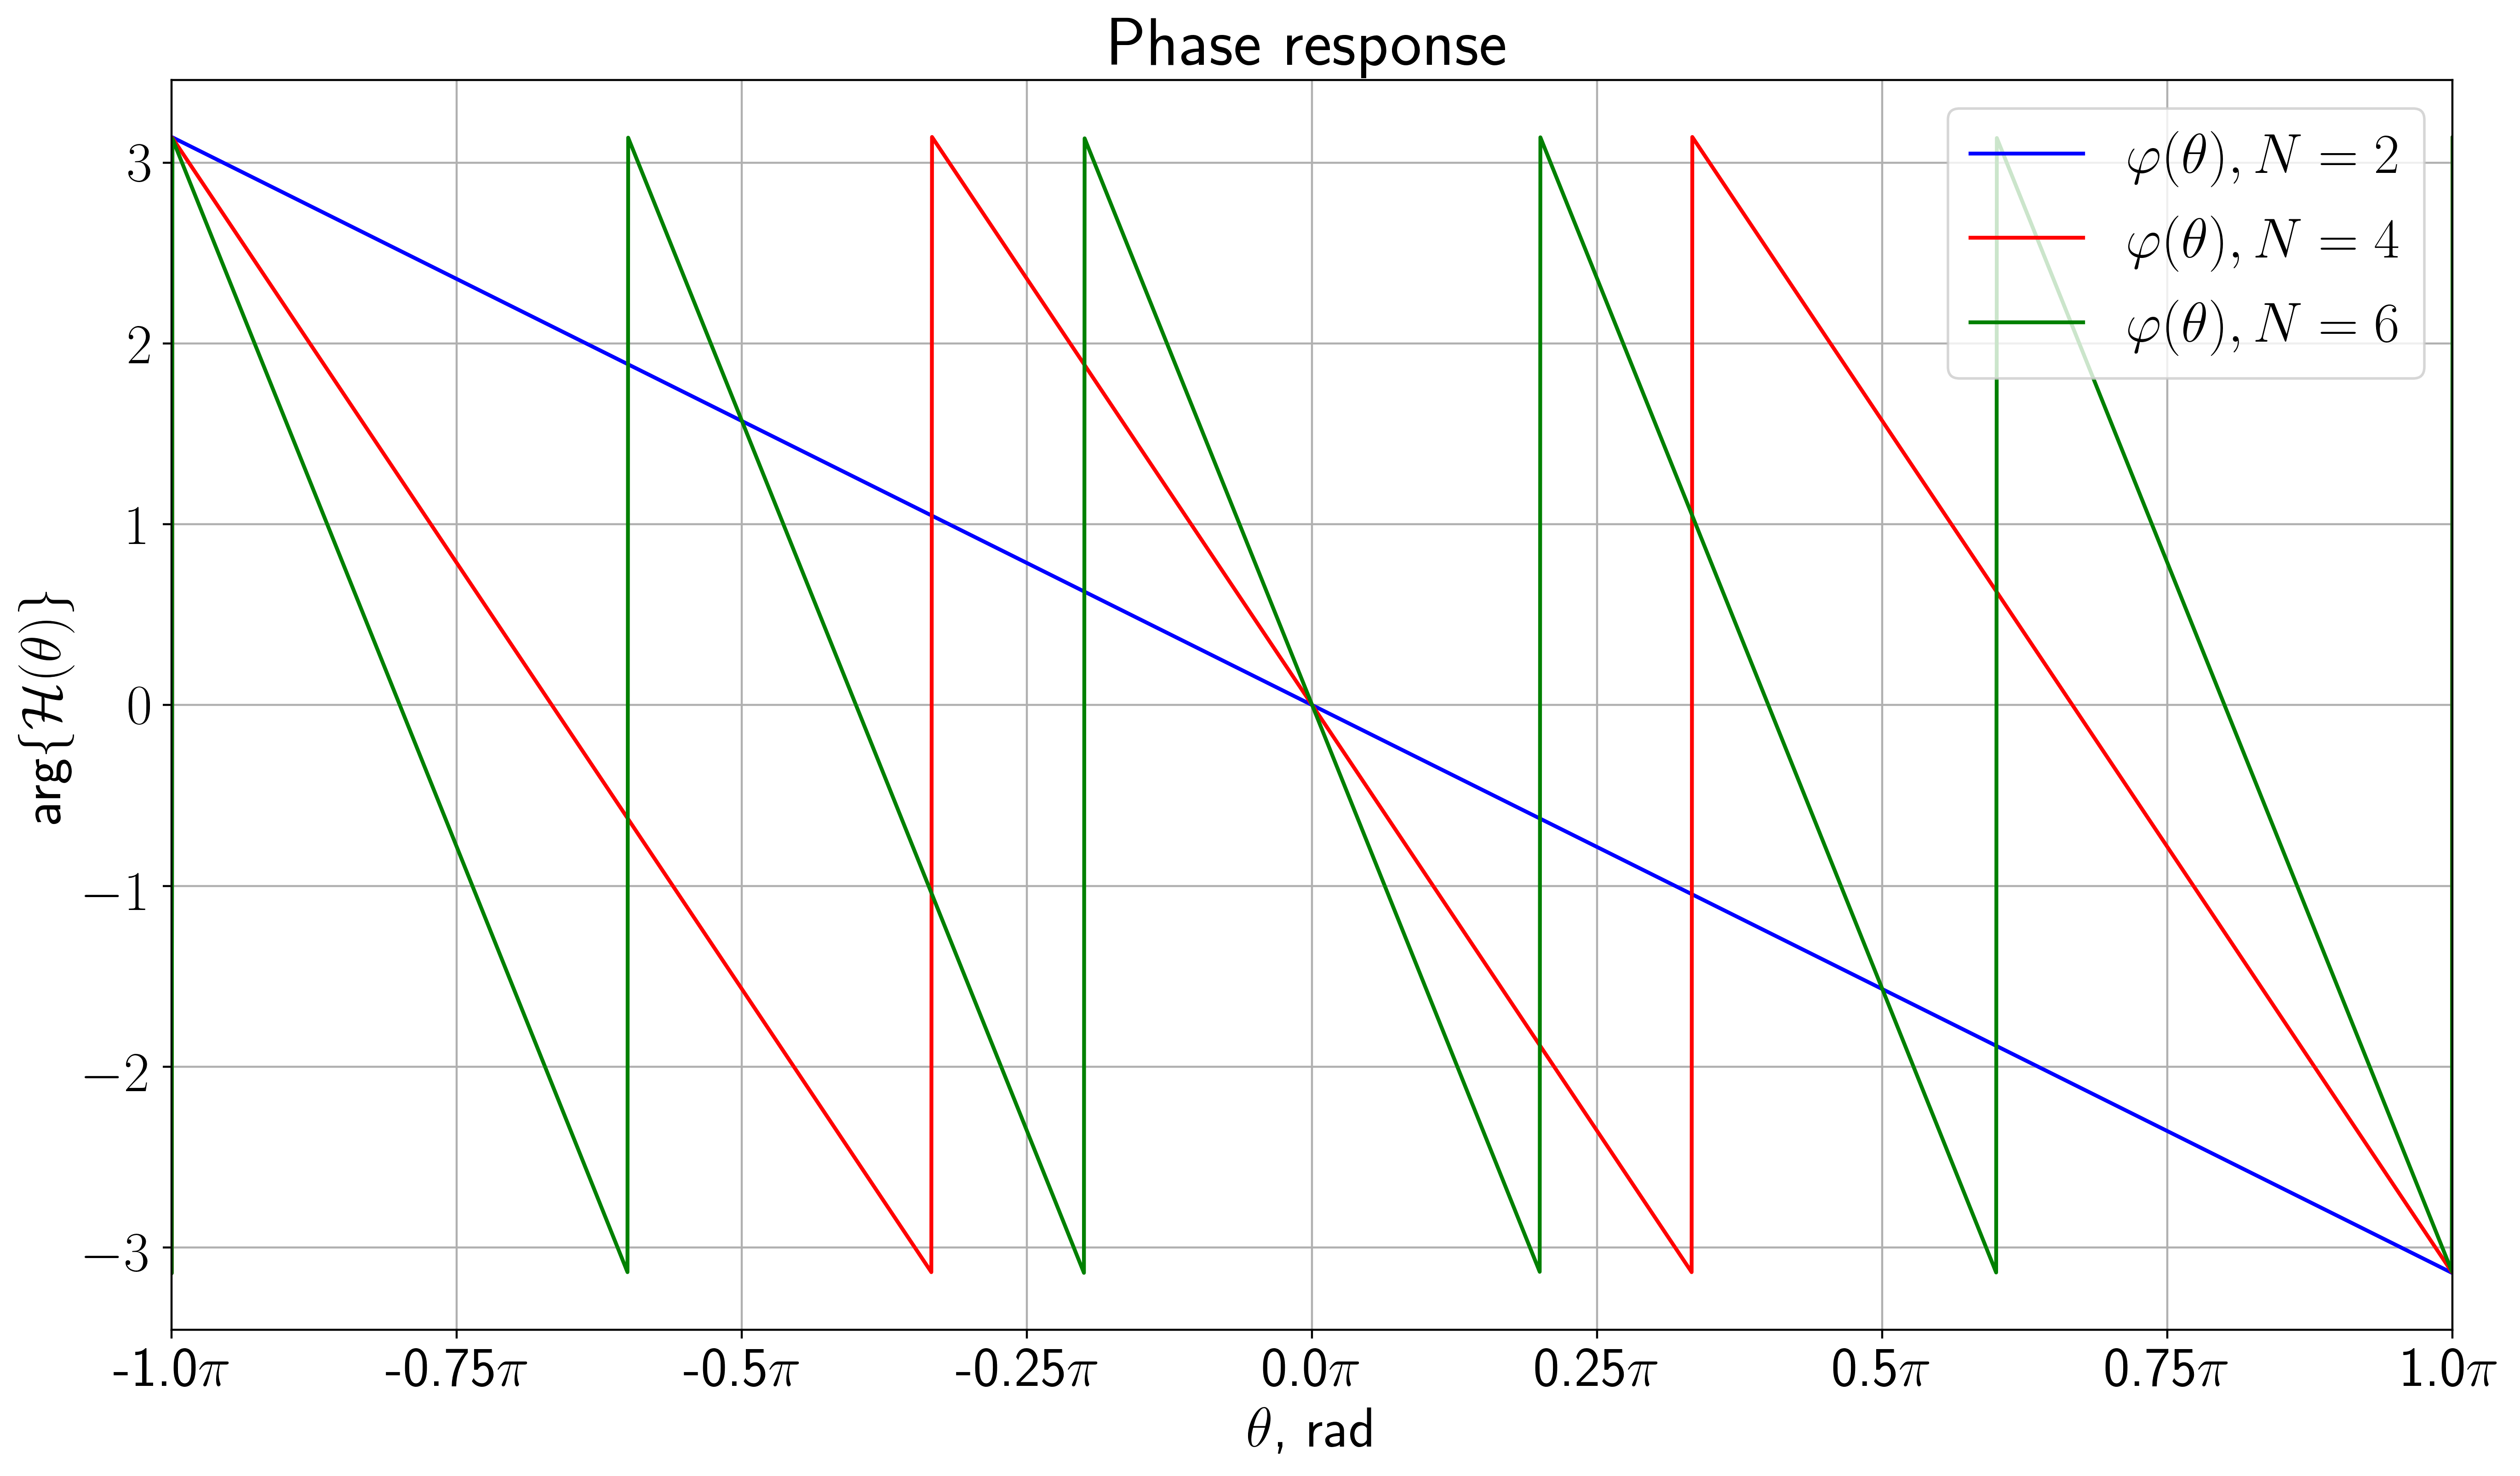
\includegraphics[width=0.8\columnwidth]{pics/fall/13/13-3.png}
	\label{fig:13-3}
\end{figure}
